\documentclass[superscriptaddress, twocolumn, prl]{revtex4}

\usepackage{amsmath}    % need for subequations
\usepackage[pdftex]{graphicx}   % need for figures
\usepackage{verbatim}   % useful for program listings
\usepackage{color}      % use if color is used in text
\usepackage{subfigure}  % use for side-by-side figures
\usepackage{hyperref}   % use for hypertext links, including those to external documents and URLs
\allowdisplaybreaks

\begin{document}

\title{The Fluid Dynamical Origin of Mammalian Ultrasonic Vocalizations}

\author{Matthew Dornfeld}
\affiliation{Laboratory of Mathematical Physics, Rockefeller University, 1230 York Ave, New York, NY 10065, USA}

\author{Diego Laplagne}
\affiliation{Shelby White and Leon Levy Center for Mind, Brain and Behavior, Rockefeller University, 1230 York Ave, New York, NY 10065, USA}

\author{Martin Elias Costa} 
\affiliation{Departamento de F\'{i}sica, FCEN, UBA Ciudad Universitaria, Pab. 1 (1428), Buenos Aires, Argentina}

\author{Marcelo Magnasco}
\affiliation{Laboratory of Mathematical Physics, Rockefeller University, 1230 York Ave, New York, NY 10065, USA}
\date{\today}
\begin{abstract}
We investigate the physical production mechanism behind mammalian narrowband ultrasonic vocalizations, using Long Evans rats as a model organism. We develop a curve fitting algorithm that extracts discontinuous jumps in frequency from many recorded calls ($n=9589$) from several rats ($N=11$). We also develop a clustering algorithm that fits this data to a fluid dynamic whistle model. By doing so we are able to conclude that the source of the vocalizations are not the vibrations of vocal folds but are the result of hole tone type whistle. A corollary of this result is that the frequency jumps are the result of an exchange in stability of flows of the whistle.
\end{abstract}
\maketitle
Although the purposes of animal vocalizations are numerous, the apparatus by which they are produced seems to be largely conserved across mammalian and bird species. This apparatus consists of membranous vocal fold tissues stretched across the larynx (or syrinx in birds). This tissue attaches to laryngeal muscles, which can alter its tension and degree of adduction. When air is forced past them, by the lungs, the vocal folds oscillate and emit audible sounds, the frequency of which are determined by the vocal fold tension. Across species, the fundamental frequencies of audible mammalian vocalizations, which span several orders of magnitude in mass, approximately obey a power law of the form $f\propto M^{-\alpha}$, where M is the species mass. However, many species of the orders Rodentia and Cetacia are known to produce narrowband ultrasonic whistles and broadband ultrasonic clicks, in addition to their sonic vocalizations. While the sonic vocalizations obey the aforementioned scaling law well, ultrasonic calls from the same species completely diverge from the power law fit by over and order of magnitude (see Fig. \ref{fig:frequency_scaling}). There is currently some debate over the exact nature of these ultrasonic calls, and the divergence from the scaling law is indicative that the production mechanism is fundamentally different from that of audible vocalizations \cite{Fletcher2010, Berke2010}.

Of the above mentioned ultrasonic vocalizations (USVs), the broadband clicks are believed to serve noncommunicative echolocative purposes. In odontocetes, the broadband clicks are known to be produced by a structure, called the phonic lips, which strike the fatty tissue of a structure called the melon, which transmits the vibrations to the surrounding water. However, The production mechanism behind the narrowband calls in cetaceans is currently unknown. Furthermore, they are believed to be directed to conspecifics for the purpose of communication. Thus, the study of these vocalizations has broader implications for the fields of animal communication and ethology as a whole \cite{Reidenberg2010}. In rodents, some experimental work has been done which discounts the possibility the narrowband calls are produced by vibrating vocal folds and indicates the production mechanism is a proper fluid dynamic whistle \cite{Riede2011,Riede2011a,Roberts1975}. However, there still does not exist a full quantitative theory of their production. It is for these reasons this paper focuses on the narrowband rodent calls and aims to provide the beginnings of a quantitative physical theory of their production by fitting recordings of narrowband vocalizations to a fluid dynamic whistle model. Because of ease of handling long-evans rats are used as a model organism. This analysis is done with the hope that the study of narrowband rodent calls will provide greater insight into those of cetaceans and animal communication in general.
\begin{figure}[!ht]
\centering
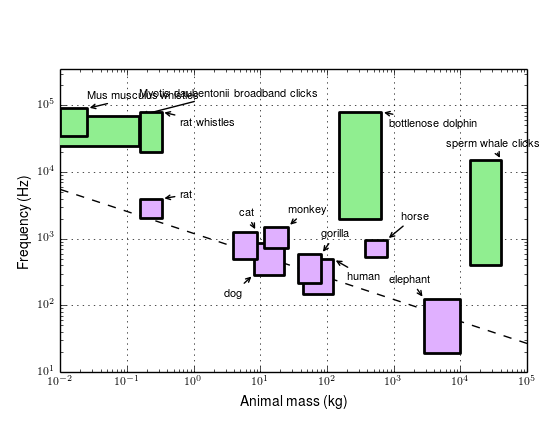
\includegraphics[width=\columnwidth]{frequency_scaling.png}
\caption{\label{fig:frequency_scaling} The purple boxes show the ranges of audible frequencies emitted by several mammals plotted against the ranges of their masses. The solid and dotted lines show plots of a frequency scaling law of the form $f\propto M^{-\alpha}$. The dotted line ($\alpha=\frac{1}{3}$) is a theoretical relationship based on the conjecture that the average frequency emitted in audible vocalizations should be inversely proportional to the linear scale of the animal. The solid line ($\alpha=0.4$) is a power law fit to the purple boxes \cite{Brudzynski2010}. The green boxes show the range of ultrasonic frequencies emitted by several mammalian species plotted against their masses \cite{white1998,berry1970natural,Fenton1998,Jones2006,bogdanowicz1994,Frankel2009,Whitehead2009,Rendell1999,Kastelein2000,Jefferson1993}.}
\end{figure}
Although several studies indicate rat USVs cannot be caused by vibrating vocal fold tissue and are likely the result of a fluid dynamic whistle, the type of whistle that constitutes this mechanism is still a point of conjecture. In general, fluid dynamic whistles consist of a jet of air, which at higher Reynolds numbers ($Re>1000$), destabilizes into a vortex street. This vortex street interacts with downstream structures, radiating acoustic energy into the far field, and inducing a velocity that provides energy to the perturbation frequencies, in the destabilized jet, which are close to the vortex shedding frequency. The perturbation frequencies with more energy become more unstable and are more likely to make contributions to the vortex street. This forms a positive feedback mechanism, which results in a fully formed vortex street with a well defined shedding frequency. The vortex street radiates acoustic energy, at a single frequency, equal to the vortex shedding rate, into the farfield. Analytic results can be obtained by neglecting the complicated destabilization process and assuming the existence of a fully formed vortex street. The equation,
\begin{equation}
\label{eq:whistle}
\frac{fL}{U_{c}}=n-\gamma,
\end{equation}
applies well to all fluid dynamic whistles that do not involve vibration of solid boundaries. The general procedure for it's derivation consists of assuming the form of the vortex street and calculating the velocity induced by the interaction of the vortex street with the downstream structure and matching its phase to that of the perturbations in the jet to ensure the positive feedback mechanism. In Eq. \ref{eq:whistle}, $f$ is the tonal frequency emitted in the acoustic far field (which is also the vortex shedding frequency), $L$ is a characteristic length scale of the system, $U_c$ is the convection velocity of the vortex street, $n$ is the acoustic mode number, and $\gamma$ is a constant that is dependent on the type of whistle. The quantity, $\frac{U_c}{f}$ is the spacing between successive vortex rings, thus $n-\gamma$ has the physical interpretation of being the number of disturbance wavelengths that can fit in the length $L$. The quantity $\gamma$ is also proportional to the phase difference between the acoustic feedback and the vortex formation rate \cite{Howe2008,Blake1986}.

It is currently unclear how rat anatomical structures would operate together as a whistle mechanism. Fig. \ref{fig:gamma_error} shows $\gamma$ for several different types of whistle mechanisms that can possibly correspond to rat anatomy. Below we will discuss how to fit data extracted from recordings of rat vocalizations to Eq. \ref{eq:whistle} to get a determination of $\gamma$, but first we will discuss how different types of whistles may correspond to rat anatomy. For the rat phonatory system to operate as an edge tone, the vocal folds would focus air coming up from the lungs into a plane jet which impinges on an edge like downstream structure- the most likely candidate for which is the junction between the nasal and bucaal cavities. A K\'{a}rm\'{a}n vortex street is then shed antisymmetrically into the nasal and bucaal cavities \cite{Holger1977,Howe2008}. However, if this were the mechanism, it would be expected that sound is emitted equally from both the nose and the mouth, and it has been observed that sound is primarily emitted from the mouth. In addition, the hole formed by the vocal folds have been observed, in anesthetized rats, by camera, to be approximately circular in shape throughout vocalization. This precludes the possibility of them focusing the stream of air into a plane jet \cite{Brudzynski2010}.  

It is also possible air emerging from the vocal folds flows over the junction to the nasal cavity into the bucaal cavity, acting as a cavity resonator. Vortices are shed at the leading edge of the opening to the nasal cavity and interact with the cavity and trailing edge to induce a velocity that radiates sound into the far field and provides acoustic feedback to reinforce vortex production at the leading edge. The analysis of cavity resonators, and thus the value of $\gamma$, depends on the ratio of the width of the cavity opening to its depth. If this ratio is less than unity, the cavity is considered shallow, and the energy stored in the cavity can be neglected. However, if the ratio is greater than unity, the cavity is considered deep, and this energy must be considered. The length of the nasal cavity is much greater than the width of the entrance to the nasal cavity at the nasal-bucaal junction. Thus, the deep cavity model seems to correspond better to rat anatomy. However, for completeness we include both values of $\gamma$ in Fig. \ref{fig:gamma_error} \cite{Howe2008, Brudzynski2010}.

The hole is tone what we believe to be the most biologically realistic model for our system. It consists of a circular jet impinging on a downstream aperture of slightly greater width. In this model, the vocal folds focus the air from lungs into a circular jet. The most likely anatomical structures for the downstream aperture are either the space between the base of the tongue and the soft palate or the one between the epiglottis and the cranial wall of the oropharynx. The circular jet destabilizes into a street of vortex rings axisymmteric about the jet axis. The vortex street causes air in the downstream aperture to oscillate, which radiates sound out of the mouth. The value of $\gamma$ in Fig. \ref{fig:gamma_error} was obtained experimentally as well as theoretically under the condition that the length between the apertures is much greater than the radius of the jet. A fact that will become important in our analysis later is this condition is not necessarily met in the rat vocal tract as the radius of the opening in the vocal folds during vocalization as well as the distance between the apertures are both on the order of 1 mm \cite{Brudzynski2010,Chanaud1965,Howe2008}.

To fit data to this model, we examined the frequency jump points from many recorded calls ($n=9589$) from eleven different rats (nine males and two females). These recordings were obtained by sampling calls at 250-300 kHz using a condenser ultrasound Avisoft-Bioacoustics CM16/CMPA-5V microphone connected to a National Instruments data acquisition card. The recordings were then divided into call snippets based on long quiescence times between vocalizations. Afterwards, the reassigned spectrogram of each call snippet was computed \cite{Gardner2006}. Since each vocalization is largely monotonal, a curve can be fitted to the call in time-frequency space by finding the frequency with the most power and computing the average of the seven frequency points surrounding and including that maximum- weighted by the amount of power in each frequency (see Fig. \ref{fig:specgram}).This is done for each time point. Jump points can then be determined by finding points where the curve rapidly changes value. For each jump point, the after frequency can be plotted against the before. The data naturally groups itself into clusters along straight lines. In doing so, we have extracted features with drastically lower dimensionality than the original data, and we hypothesize that each cluster corresponds to one type of mode transition, with $n\rightarrow n\pm1$. 
\begin{figure}[!ht]
\centering
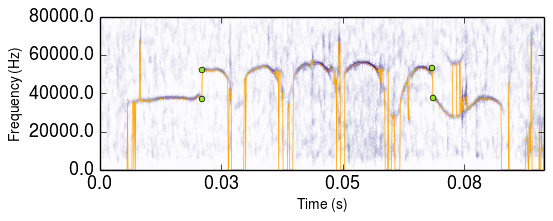
\includegraphics[width=\columnwidth]{specgram.png}
\caption{\label{fig:specgram} Reassigned spectrogram of a segment of a rat USV. The orange line is the output of the curve fitting algorithm. The green circles show the output of the jump extraction algorithm.}
\end{figure}
To fit the extracted jump points to Eq. \ref{eq:whistle} we developed a clustering algorithm, which as input, accepts a list of slopes of straight lines. The number of clusters in the output is equal to the length of the list. The algorithm then iterates over each jump point in the dataset and computes the perpendicular distance of the point to the line defined by each slope. The point is then assigned to the line for which this value is minimum. If $\left(f_{1},\: f_{2}\right)$ and $\left(n,\: n\pm1\right)$ are the frequencies and mode numbers before and after a jump respectively, by dividing the after jump frequency mode relation by the before jump relation, we get 
\begin{equation}
\label{eq:freqmode2}
\frac{f_{2}}{f_{1}}=m(c,\gamma)=\frac{n\pm1-\gamma}{n-\gamma},
\end{equation}where $c$ is the cluster to which that jump has been assigned, and $\left(n,\: n\pm1\right)$ is a function of the cluster. Several mode transitions were experimented with to best fit the data. In the extracted jumps, we found transitions in mode numbers ranging from $n=2$ to $n=6$. The $n=1$ mode seems to correspond to 22-kHz alarm calls, which do not exhibit jumps as often and therefore are not represented in our dataset. Not all rats in our study produced enough jumps in all mode regions to fit the data to our algorithm, so underpopulated modes were excluded for some rats. Eq. \ref{eq:freqmode2} can then be used to generate the slopes needed as input for the algorithm.

We can define a cost function that adds up the squares of the perpendicular distances of each point to their assigned line. 
\begin{align*}
\Delta x_{i_{c}} &= \left\vert f_{1,i_{c}}-\frac{f_{1,i_{c}}+m\left(c,\gamma\right)f_{2,i_{c}}}{m\left(c,\gamma\right)^{2}+1}\right\vert
\\ \Delta y_{i_c} &= \left\vert f_{2,i_{c}}-\frac{m\left(c,\gamma\right)\left(f_{1,i_{c}}+m\left(c,\gamma\right)f_{2,i_{c}}\right)}{m\left(c,\gamma\right)^{2}+1}  \right\vert
\end{align*}
\begin{equation}
\label{eq:cost}
C\left(\gamma\right)=\sum_{c}\frac{1}{N_{c}}\sum_{i_c=1}^{N_{c}}\left(\Delta x_{i_c}\right)^{2}+\left(\Delta y_{i_c}\right)^{2},
\end{equation}
where $\Delta x_{i_c}$ and $\Delta y_{i_c}$ are the respective horizontal and vertical distances of the $i^{th}$ point in cluster $c$ to its assigned line, and $N_{c}$ is the number of points in cluster $c$. By minimizing Eq. \ref{eq:cost} over $\gamma$, we can get a determination for which cluster each point belongs to as well as a numerical calculation for the value $\gamma$. 
\begin{figure}[!ht]
\centering
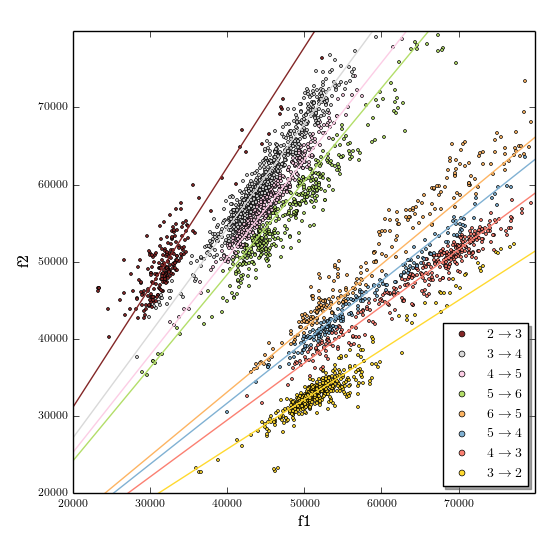
\includegraphics[width=\columnwidth]{V4.png}
\caption{\label{fig:jumps}After jump frequency plotted against before jump frequency for jumps extracted from V4. The points are color coded according to the transition cluster they were assigned by the clustering algorithm. The legend in the bottom right shows which mode transitions ($n\rightarrow n\pm1$) correspond to the color. The lines are plots of Eq. \ref{eq:freqmode2}, for $\gamma=\gamma_{min}^{V4}$ and obey the same color coding scheme.} 
\end{figure}

Fig. \ref{fig:jumps} shows the output of the clustering algorithm, for the rat V4, for, $\gamma=\gamma_{min}^{V4}$, the values of $\gamma$ that minimize Eq. \ref{eq:cost} for a given rat, along with plots, of the lines defined by $m\left(c,\gamma_{min}^{V4}\right)$, for each cluster \cite{jump_appendix}. We also experimented with adding a parameter that offset the lines defined by Eq. \ref{eq:freqmode2} from the origin. As expected, in all cases, it was found to be effectively zero, so we do not include it in further analysis. The data in Fig. \ref{fig:jumps} is grouped into eight clusters- four that correspond to up transitions and four that correspond to down transitions. Unlike some other rats used in this study, V4 exhibits a significant number of jump points in the $2\rightarrow3$ and $3\rightarrow2$ transition clusters, which are mostly populated by jumps between constant frequency calls in the 30 kHz range to constant frequency calls in the 50 kHz and vice versa, which were rarely recorded for an unknown reason. These clusters are noticeably distinct from the others and can be separated out by visual inspection. The clusters that represent transitions between higher regions present more of an overlap with each other. The $3\rightarrow4$, $5\rightarrow6$, $4\rightarrow3$, and $6\rightarrow5$ clusters show clear drop offs in density at their borders, which seems to be well represented in the output of the algorithm. However, the $4\rightarrow5$ and $5\rightarrow4$ transition clusters do not seem to be well represented in the data for this rat. Thus, it is hard to identify these clusters based on visual inspection of the density of jump points, although we still believe them to be present in smaller numbers. It is also worth noting that, removing those clusters from the algorithm did not produce a significant change in the calculated value of $\gamma$. 
\begin{figure}[!ht]
\centering
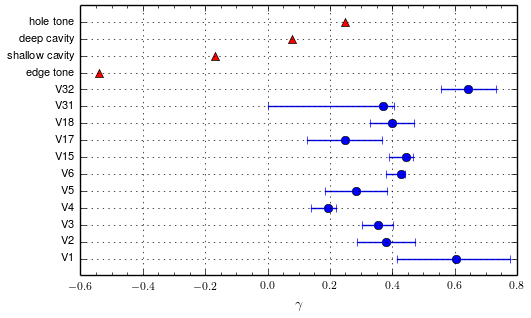
\includegraphics[width=\columnwidth]{gamma_error.png}
\caption{\label{fig:gamma_error} The blue shows $\gamma_{min}^{rat}$ along with 95 \% confidence intervals obtained from bootstrap analysis. The red shows values of $\gamma$ known for several whistle types \cite{Howe2008}.}
\end{figure}
The results of Figs. \ref{fig:jumps} and \ref{fig:gamma_error} give clear indications about the nature of the whistle mechanism underlying narrowband USVs. Upon inspection of Fig.\ref{fig:jumps} evidence of hysteresis can be seen as the densities of opposite transition clusters are not mirror images of each other and seem to be translated and warped along the lines with slope $m\left(c,\gamma_{min}^{rat}\right)$, which would be expected for a fluid dynamic whistle. Furthermore, the points of each cluster seem to be distributed roughly symmetrically around these lines. This indicates the frequency jumps are the result of a noisy process in the vicinity of a critical point of the system, which would also be expected for a whistle system. Fig. \ref{fig:gamma_error} shows a comparison of the values of $\gamma_{min}$ obtained for the rats used in this study with ones known for different fluid dynamic whistles. Based on these results, we can conclusively rule out the edge tone, shallow cavity, and deep cavity mechanisms as being the source of rat USVs. The values of $\gamma$ obtained from this study correspond best with the one known for the hole tone. Although this correspondence is not exact, we believe it supports our conjecture that the underlying mechanism for USVs is hole tone like. Furthermore, as mentioned above, the value of $\gamma$ known for the hole tone was obtained under the condition that the length between the up and downstream apertures is much greater than the radius of the jet. A condition that we do not believe is met in the rat vocal tract and would imply that fewer disturbance wavelengths fit in the length $L$, which correspond to a larger value of $\gamma$. In addition, the resonant properties of the upper vocal tract would also affect the value obtained for $\gamma$. We believe further theoretical analysis, using these assumption, would produce values $\gamma$ in agreement our data.
\bibliographystyle{prsty}
\bibliography{mdornfe1.bib}

\appendix
\section{\label{App:add_data}Appendix: Additional Data}
\begin{figure*}[ht]
\centering
\subfigure{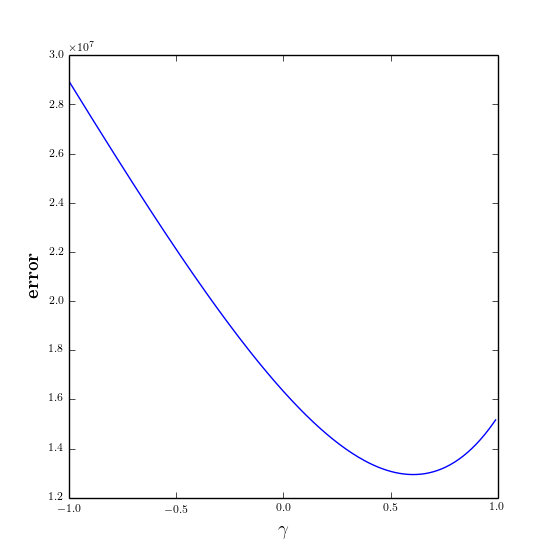
\includegraphics[width=\columnwidth]{figs/error_V1.png}}
\subfigure{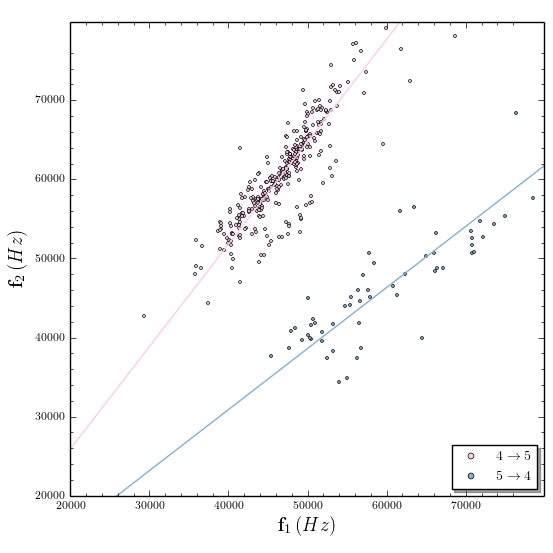
\includegraphics[width=\columnwidth]{figs/V1.png}}
\caption{For rat V1, left shows plot of Eq. \ref{eq:cost} as a function of $\gamma$. Right shows output of clustering algorithm with $\gamma$ equal to the value shown in Fig. \ref{fig:gamma_error}.}
\end{figure*}

\begin{figure*}[h]
\centering
\subfigure{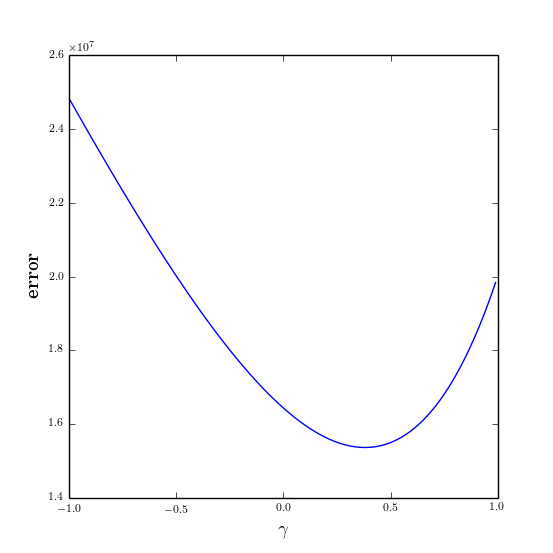
\includegraphics[width=\columnwidth]{figs/error_V2.png}}
\subfigure{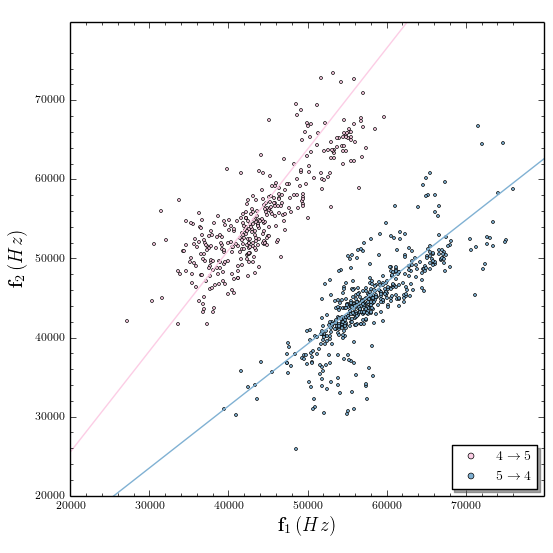
\includegraphics[width=\columnwidth]{figs/V2.png}}
\caption{For rat V2, left shows plot of Eq. \ref{eq:cost} as a function of $\gamma$. Right shows output of clustering algorithm with $\gamma$ equal to the value shown in Fig. \ref{fig:gamma_error}.}
\end{figure*}

\begin{figure*}
\centering
\subfigure{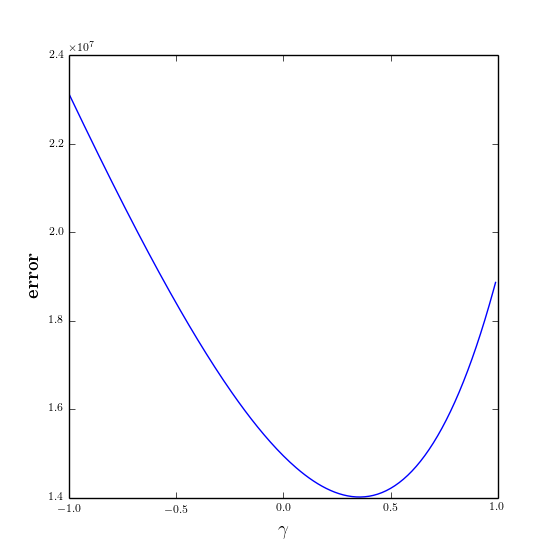
\includegraphics[width=\columnwidth]{figs/error_V3.png}}
\subfigure{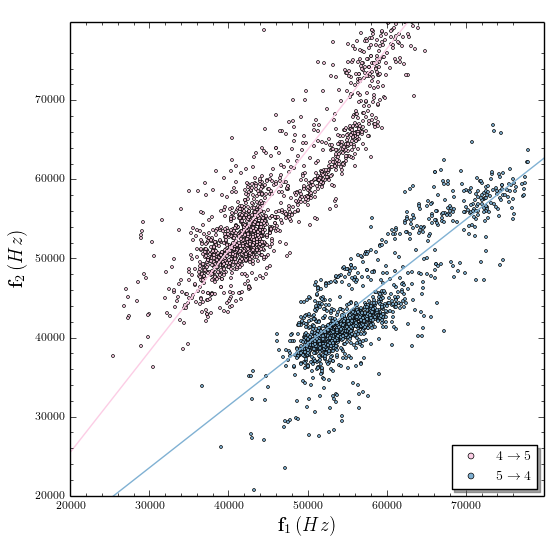
\includegraphics[width=\columnwidth]{figs/V3.png}}
\caption{For rat V3, left shows plot of Eq. \ref{eq:cost} as a function of $\gamma$. Right shows output of clustering algorithm with $\gamma$ equal to the value shown in Fig. \ref{fig:gamma_error}.}
\end{figure*}

\begin{figure*}
\centering
\subfigure{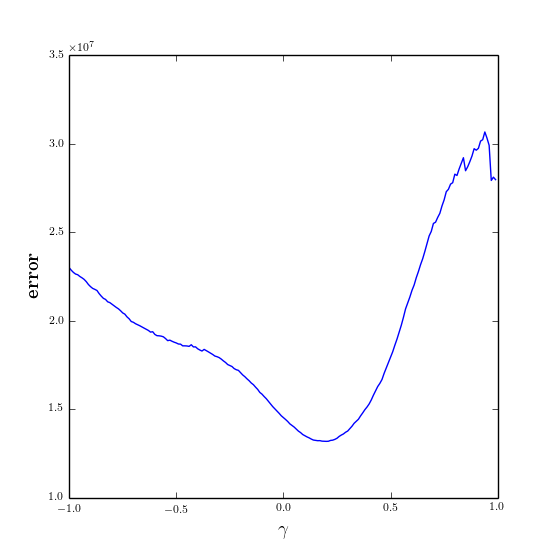
\includegraphics[width=\columnwidth]{figs/error_V4.png}}
\subfigure{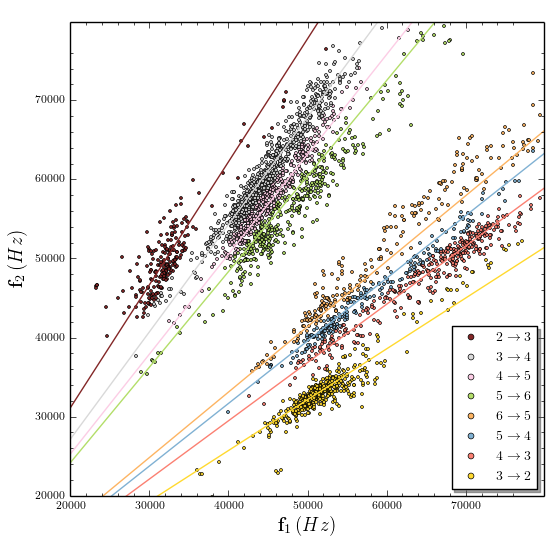
\includegraphics[width=\columnwidth]{figs/V4.png}}
\caption{For rat V4, left shows plot of Eq. \ref{eq:cost} as a function of $\gamma$. Right shows output of clustering algorithm with $\gamma$ equal to the value shown in Fig. \ref{fig:gamma_error}.}
\end{figure*}

\begin{figure*}
\centering
\subfigure{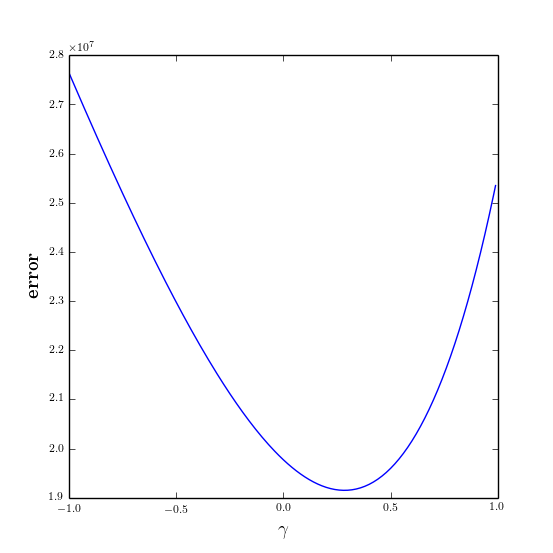
\includegraphics[width=\columnwidth]{figs/error_V5.png}}
\subfigure{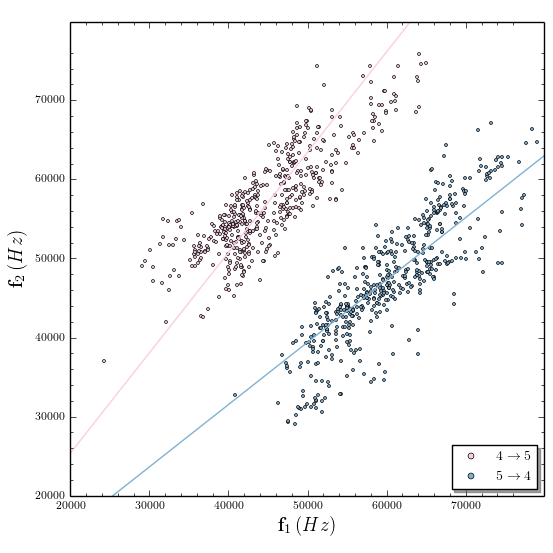
\includegraphics[width=\columnwidth]{figs/V5.png}}
\caption{For rat V5, left shows plot of Eq. \ref{eq:cost} as a function of $\gamma$. Right shows output of clustering algorithm with $\gamma$ equal to the value shown in Fig. \ref{fig:gamma_error}.}
\end{figure*}

\begin{figure*}
\centering
\subfigure{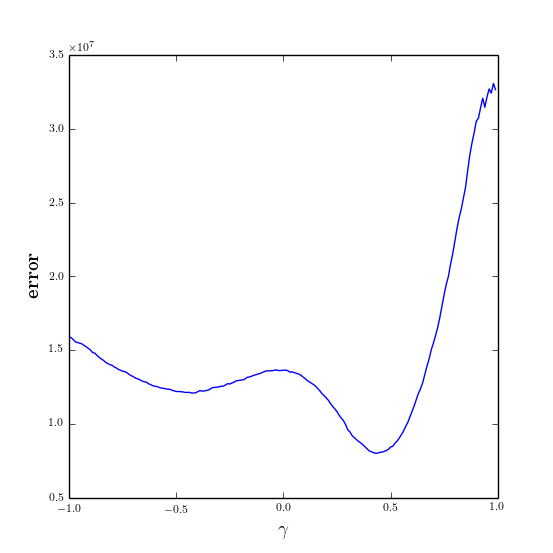
\includegraphics[width=\columnwidth]{figs/error_V6.png}}
\subfigure{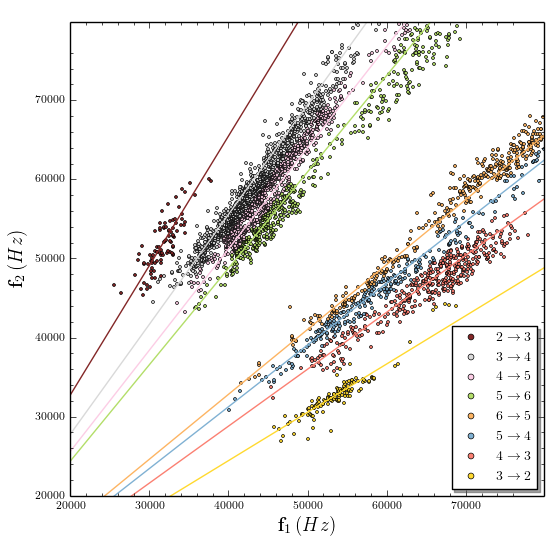
\includegraphics[width=\columnwidth]{figs/V6.png}}
\caption{For rat V6, left shows plot of Eq. \ref{eq:cost} as a function of $\gamma$. Right shows output of clustering algorithm with $\gamma$ equal to the value shown in Fig. \ref{fig:gamma_error}.}
\end{figure*}

\begin{figure*}
\centering
\subfigure{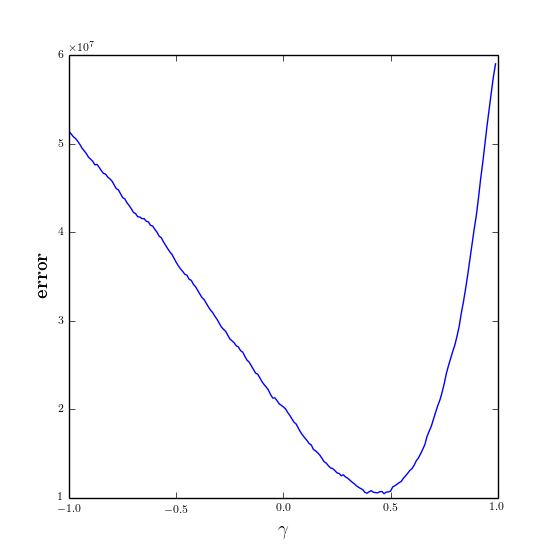
\includegraphics[width=\columnwidth]{figs/error_V15.png}}
\subfigure{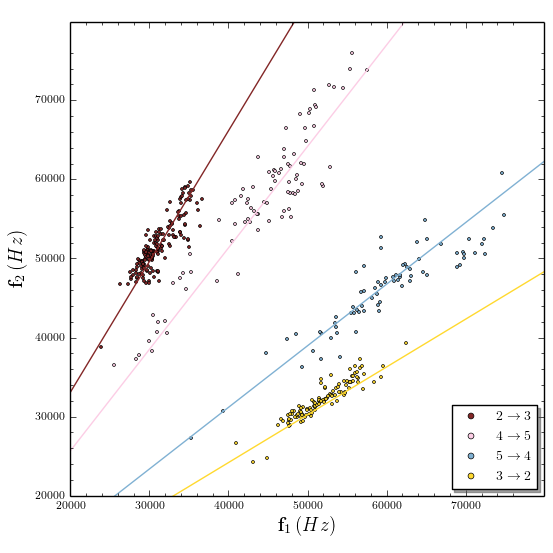
\includegraphics[width=\columnwidth]{figs/V15.png}}
\caption{For rat V15, left shows plot of Eq. \ref{eq:cost} as a function of $\gamma$. Right shows output of clustering algorithm with $\gamma$ equal to the value shown in Fig. \ref{fig:gamma_error}.}
\end{figure*}

\begin{figure*}
\centering
\subfigure{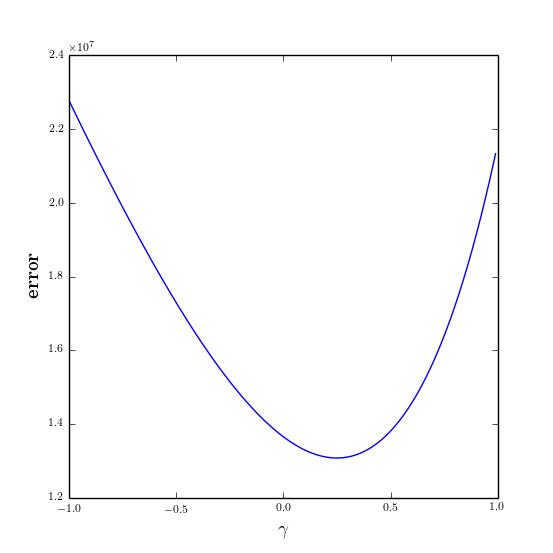
\includegraphics[width=\columnwidth]{figs/error_V17.png}}
\subfigure{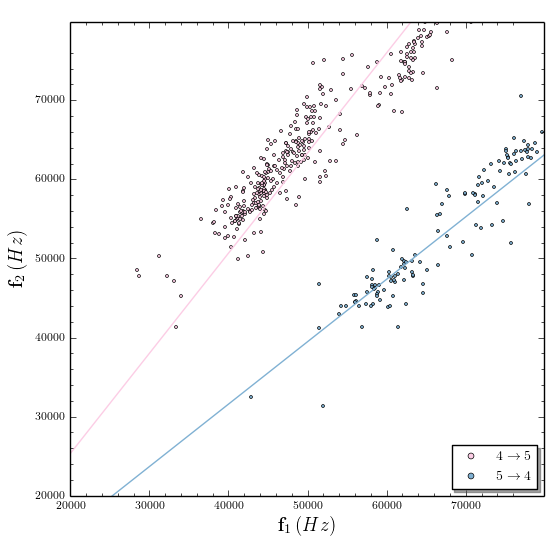
\includegraphics[width=\columnwidth]{figs/V17.png}}
\caption{For rat V17, left shows plot of Eq. \ref{eq:cost} as a function of $\gamma$. Right shows output of clustering algorithm with $\gamma$ equal to the value shown in Fig. \ref{fig:gamma_error}.}
\end{figure*}

\begin{figure*}
\centering
\subfigure{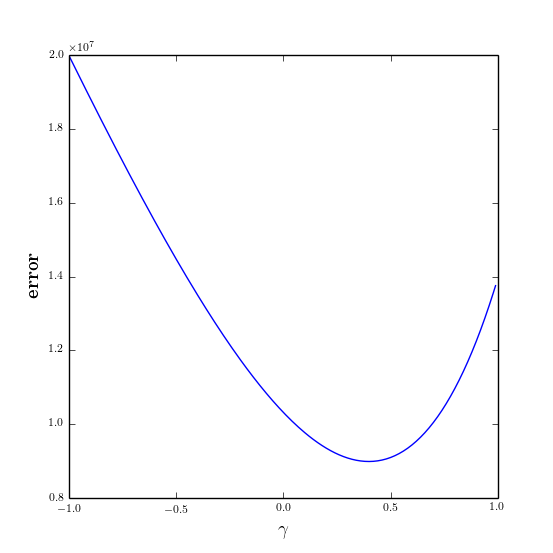
\includegraphics[width=\columnwidth]{figs/error_V18.png}}
\subfigure{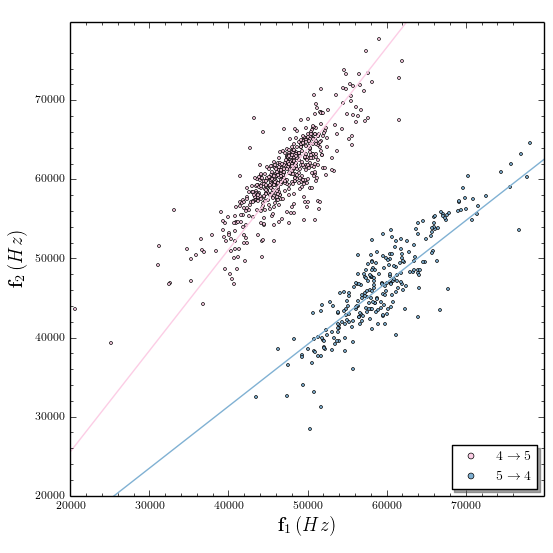
\includegraphics[width=\columnwidth]{figs/V18.png}}
\caption{For rat V18, left shows plot of Eq. \ref{eq:cost} as a function of $\gamma$. Right shows output of clustering algorithm with $\gamma$ equal to the value shown in Fig. \ref{fig:gamma_error}.}
\end{figure*}

\begin{figure*}
\centering
\subfigure{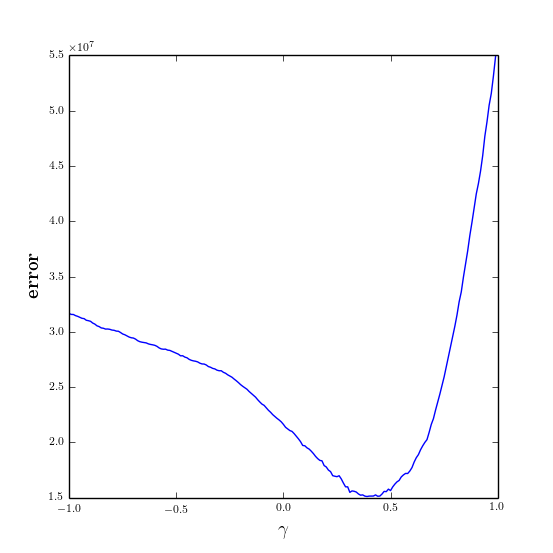
\includegraphics[width=\columnwidth]{figs/error_V31.png}}
\subfigure{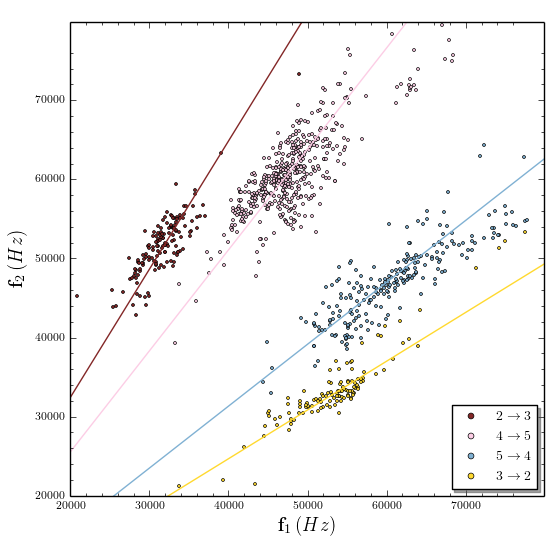
\includegraphics[width=\columnwidth]{figs/V31.png}}
\caption{For rat V31, left shows plot of Eq. \ref{eq:cost} as a function of $\gamma$. Right shows output of clustering algorithm with $\gamma$ equal to the value shown in Fig. \ref{fig:gamma_error}.}
\end{figure*}

\begin{figure*}
\centering
\subfigure{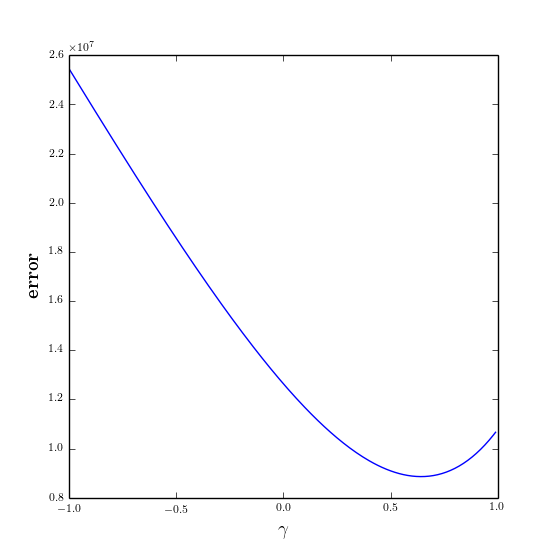
\includegraphics[width=\columnwidth]{figs/error_V32.png}}
\subfigure{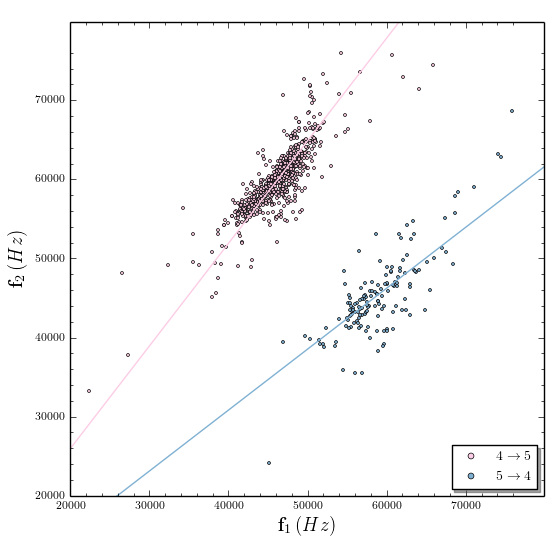
\includegraphics[width=\columnwidth]{figs/V32.png}}
\caption{For rat V32, left shows plot of Eq. \ref{eq:cost} as a function of $\gamma$. Right shows output of clustering algorithm with $\gamma$ equal to the value shown in Fig. \ref{fig:gamma_error}.}
\end{figure*}
\end{document}

